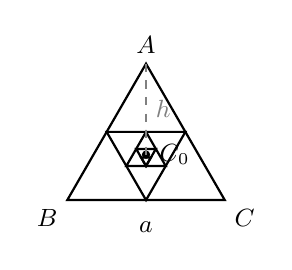
\begin{tikzpicture}[scale=1, font=\small]
  % 无限内接等边三角形框架 (Problem 5-1)
  % Outermost triangle ABC with side length a
  \coordinate (A) at (0, 1.732);
  \coordinate (B) at (-1, 0);
  \coordinate (C) at (1, 0);

  % Draw outer triangle
  \draw[thick] (A) -- (B) -- (C) -- cycle;

  % Labels for outer vertices
  \node[above] at (A) {$A$};
  \node[below left] at (B) {$B$};
  \node[below right] at (C) {$C$};

  % Side label
  \node[below] at (0, -0.15) {$a$};

  % First inner triangle (midpoints of outer)
  \coordinate (AB) at (-0.5, 0.866); % midpoint of AB
  \coordinate (BC) at (0, 0);          % midpoint of BC
  \coordinate (CA) at (0.5, 0.866);   % midpoint of CA

  \draw[thick] (AB) -- (BC) -- (CA) -- cycle;

  % Second inner triangle
  \coordinate (AB_BC) at (-0.25, 0.433); % midpoint of AB-BC edge
  \coordinate (BC_CA) at (0.25, 0.433);  % midpoint of BC-CA edge
  \coordinate (CA_AB) at (0, 0.866);     % midpoint of CA-AB edge (top)

  \draw[thick] (AB_BC) -- (BC_CA) -- (CA_AB) -- cycle;

  % Third inner triangle
  \coordinate (p1) at (-0.125, 0.6495);
  \coordinate (p2) at (0.125, 0.6495);
  \coordinate (p3) at (0, 0.433);

  \draw[thick] (p1) -- (p2) -- (p3) -- cycle;

  % Fourth inner triangle (smallest visible)
  \coordinate (q1) at (-0.0625, 0.5413);
  \coordinate (q2) at (0.0625, 0.5413);
  \coordinate (q3) at (0, 0.433);

  \draw[thick] (q1) -- (q2) -- (q3) -- cycle;

  % Center of mass mark
  \fill (0, 0.577) circle (1.5pt);
  \node[right] at (0.05, 0.577) {$C_0$};

  % Height line from A to center of mass
  \draw[dashed, gray] (A) -- (0, 0.577) node[midway, right] {$h$};
\end{tikzpicture}
